\documentclass{home_assignment}
\begin{document}
    \titlePage{Propagation and Antenna Assignment \#1}{October 10, 2020}{Ram Krishna Maharjan, Ph.D.}
    \problem{Smart Antennas}
    \solution{A smart antenna is one that is able to respond to its electromagnetic environment in such a way that it improves a certain performance criterion such as increased immunity to signal interference, or reduced signal level for a vulnerable receiver. A smart antenna has the capability of focusing on a desired user while rejecting unwanted signals giving it a low bit error rate (BER). A smart antenna is a system
    involving multiple antenna elements and a digital signal processor to adjust the radiation.The concept of smart antennas was first implemented in switched-beam system, which has some demerits that led to the advent of an adaptive array system. 
    \subsection*{Switched-Beam System}
    This is the simplest form of a smart antenna. It uses multiple fixed beams with elevated sensitivity in certain directions. The system chooses from one of multiple predetermined fixed beams and switches from one beam to other as the device moves along the radition pattern. This system is based on a generic switching technique and can select the strongest signal to be received. Since each sector is subdivided into smaller sectors, this section is generally referred to as the extension to cell sectoring. The static natire of the beams meant that the users had trouble depending on their locations if it wasn't exactly centered on the active beam. This gave the interfering signal more enhancement than the desired signal. 
    \begin{figure}[H]
        \centering
        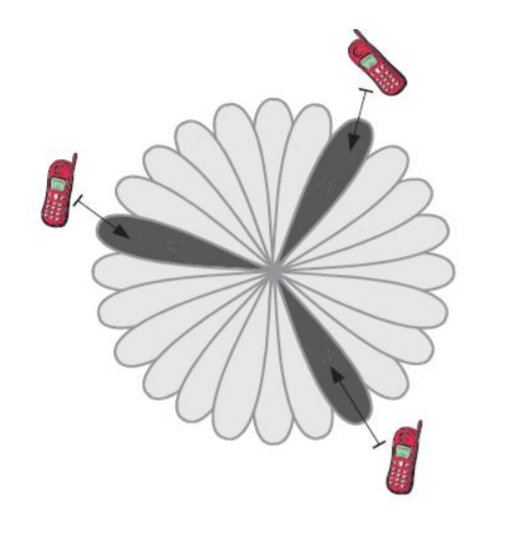
\includegraphics[scale=0.9]{Figures/switchedbeam.png}
        \caption{Switched-beam coverage pattern}
        \label{fig:switchedbeam}
    \end{figure}
    \subsection*{Adaptive Array System}
    The adaptive antenna systems communicates between a user and a base by adding the dimension of space. By adjusting to the RF
    environment as it changes, adaptive antenna technology can dynamically alter the signal patterns to optimize the performance of the wireless system. The switched-beam system is not able to place the desired signal at the maximum of the main
    lobe, and it exhibits inability to reject the interferers fully. Because of the ability to control
    the overall radiation pattern in a greater coverage area for each cell site, as illustrated in
    Figure \ref{fig:comparision}, adaptive array systems can provide great increase in capacity. Adaptive array
    systems can locate and track signals (users and interferers) and dynamically adjust the
    antenna pattern to enhance reception while minimizing interference using signal processing
    algorithms.
    \begin{figure}[H]
        \centering
        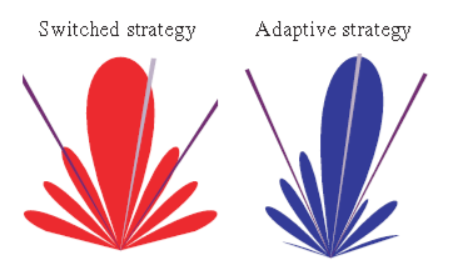
\includegraphics[]{Figures/smart_antennas.png}
        \caption{Beam formations of different systems of smart antennas}
        \label{fig:comparision}
    \end{figure}
    }
    \problem{Give some important control points which can be used to design any kinds of array antennas. Find out the transmitting power in watt, if overall EIRP of the communication system is calculated 52 dBW for transmitting central frequency 4.2 GHz of 36 MHz bandwidth and use 6.4 m diameter transmitting antenna with 82 percent its efficiency, as well as 1.8 dB cable loss is considered.}
    \solution{
        \subsubsection*{Part I}
        The important control points that can be used to design any kinds of array antennas are:
    \begin{enumerate}
        \item \textbf{Array Factor:} It is calculated as a function of the excitation to each and every element and arrangements of elements in the array. The array factor AF of a linear array antenna can be calculated as,\begin{equation}
            AF(\theta)=\sum_{n=1}{N}e^{j(n-1)(kdcos\theta)+\Psi}
        \end{equation}
        where, $AF(\theta)$ is the Array Factor w.r.t $\theta$\\
        $k=2\pi/\lambda$,\\
        $d$ is the distance between the two elements in the array,\\$\Psi$ is the phase shift,\\
        $N$ is the Number of elements in the array antenna
        \item \textbf{Array Pattern:} This is the resultant of the simple multiplication of the array factor with the radiation pattern of individual element. 
        \begin{equation}
            \text{Array Pattern=Array factor x Radiation pattern of single element}
        \end{equation}
    \end{enumerate}
    \subsubsection*{Part II}
    Given values are,\\
    Frequency$(f)=4.2 GHz\Rightarrow \lambda=\frac{c}{f}=\frac{3 \times 10^8}{4.2 \times 10^8}=0.0714$,\\
    Diameter$(d)=6.4m$,\\
    Cable Loss$(L_c)=1.8 dB$,\\
    $EIRP=52dBW$,\\
    Efficiency$(\eta)=0.82$\\
    We have the relation for $EIRP$,
    \begin{equation}
        EIRP=P_T(dBW)+G_{TX}(dBi)-L_c(dB)
        \label{eqn:EIRP}
    \end{equation}
    Also, the relation for transmitting antenna in dB is,
    \begin{equation}
        G_{TX}=10 \quad log_{10}\left(\eta\frac{\pi d^2}{\lambda^2}\right)
        \label{eqn:gain}
    \end{equation}
    Putting values of $\lambda$, $\pi$, $d$ and $\eta$ in Equation \ref{eqn:gain} we get,
    \begin{equation*}
        G_{TX}=43.1558\quad dBi
    \end{equation*}
    Putting the value of $G_{TX}$, $L_c$ and $EIRP$ in Equation \ref{eqn:EIRP},
    \begin{equation*}
        \begin{aligned}
            P_T(dBW)&=52+1.8-43.1558\\
            &=10.64420\quad dBW\\
            P_T(W)&=10^{\left(\frac{10.64420}{10}\right)}\\
            P_T(W)&=11.59899 \quad W
        \end{aligned}
    \end{equation*}
    Thus, the transmitting power is 11.59899 $W$.
    }
\end{document}